\documentclass{article}
\usepackage{graphicx}
\usepackage{amsmath}
\usepackage{amsfonts}
\usepackage{bookmark}
\usepackage{booktabs}
\usepackage{exercises}
\graphicspath{ {./images/test} }
\usepackage{indentfirst}
\usepackage{amsthm}
\usepackage{yhmath}
\usepackage{geometry}
\usepackage{placeins}
\usepackage{csquotes}
\usepackage{pgfplots}
\newcommand*{\oldneg}{\mathord{\sim}}
\newcommand\showdiv[1]{\overline{\smash{)}#1}}
\newcommand\Mydiv[1]{%
\smash{\raise.3ex\hbox{$\big)$}}\mkern-8mu
        \overline{\enspace\strut#1}}
\setlength{\tabcolsep}{5pt}
\theoremstyle{definition}
\newtheorem{definition}{Definition}

\setlength{\parindent}{.5in}
\setlength{\parskip}{12pt}
\renewcommand{\arraystretch}{2}
\geometry{margin=1in}
\newcommand{\?}{\stackrel{?}{=}}
\pgfplotsset{width=7cm,compat=1.18}\usepgfplotslibrary{statistics}

\title{Chapter 8 Test (pg. 549)}
\begin{document}
\maketitle

\section*{1}
The distance is $\sqrt{(7+1)^2-(3-5)^2}=\sqrt{64-4}=\sqrt{60}=2\sqrt{15}$.
The midpoint of the segment joining the two points is $(\frac{-1+7}{2},\frac{5+3}{2})=(3,4)$.

\section*{2}
The distance is $\sqrt{(8-4)^2+(8-2)^2}=\sqrt{16+36}=\sqrt{52}=2\sqrt{13}$.
The midpoint of the segment joining the two points is $(\frac{4+8}{2},\frac{2+8}{2})=(6,5)$.

\section*{3}
The distance is $\sqrt{(1+1)^2+(5+6)^2}=\sqrt{4+121}=\sqrt{125}=5\sqrt{5}$.
The midpoint of the segment joining the two points is $(\frac{-1+1}{2},\frac{-6+5}{2})=(0,-\frac{1}{2})$.

\section*{4}
The distance is $\sqrt{(3-2)^2+(1+5)^2}=\sqrt{1+36}=\sqrt{37}$.
The midpoint of the segment joining the two points is $(\frac{2+3}{2},\frac{-5+1}{2})=(\frac{5}{2},-2)$.

\section*{5}
The distance is $\sqrt{(-3+6)^2+(5+2)^2}=\sqrt{9+49}=\sqrt{58}$.
The midpoint of the segment joining the two points is $(\frac{-6-3}{2},\frac{-2+5}{2})=(-\frac{9}{2},\frac{3}{2})$.

\section*{6}
The distance is $\sqrt{(10-1)^2+(-2-9)^2}=\sqrt{81+121}=\sqrt{202}$.
The midpoint of the segment joining the two points is $(\frac{1+10}{2},\frac{9-2}{2})=(\frac{11}{2},\frac{7}{2})$.

\section*{7}
We are given the equation \[ y^2-24x=0 \] \[ y^2=24x \] meaning this is a parabola with a horizontal axis of symmetry. We know that $p=\frac{24}{4}=6$, and thus the focus is 
$(6,0)$ and the directrix is $x=-6$:\newline
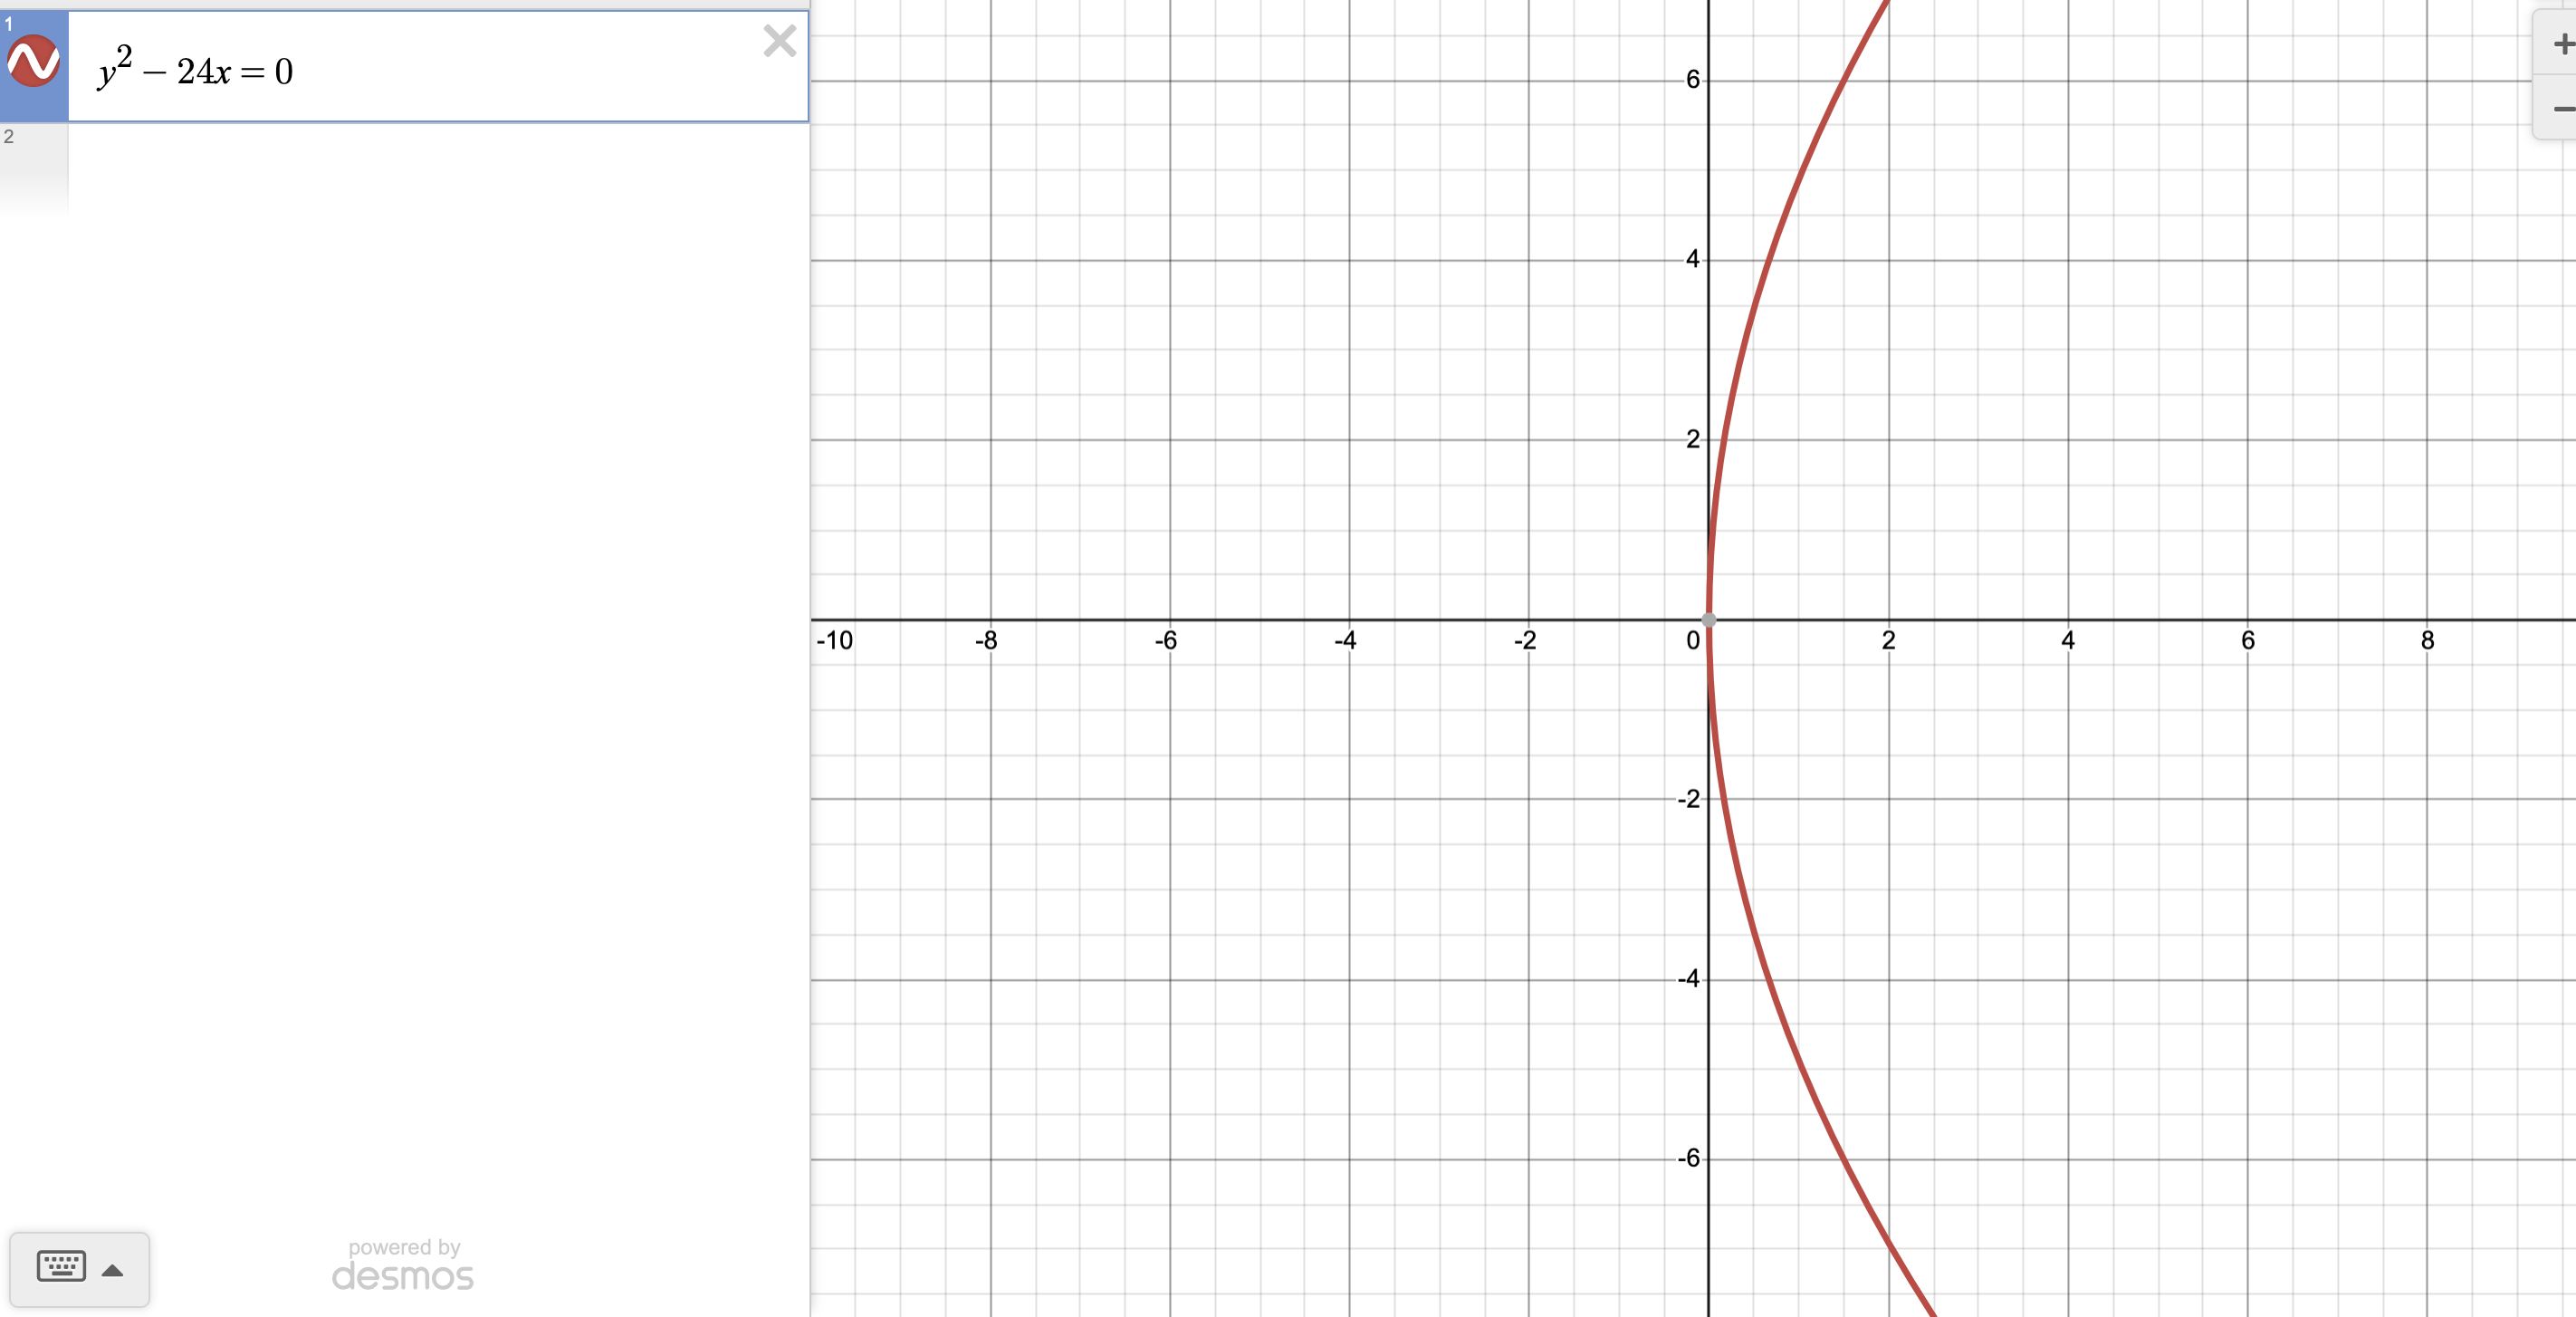
\includegraphics[width = 4in]{7}

\section*{8}
We are given the equation \[ x^2+y^2=16=4^2 \] meaning this is a circle centered at the origin with a radius of 4:\newline
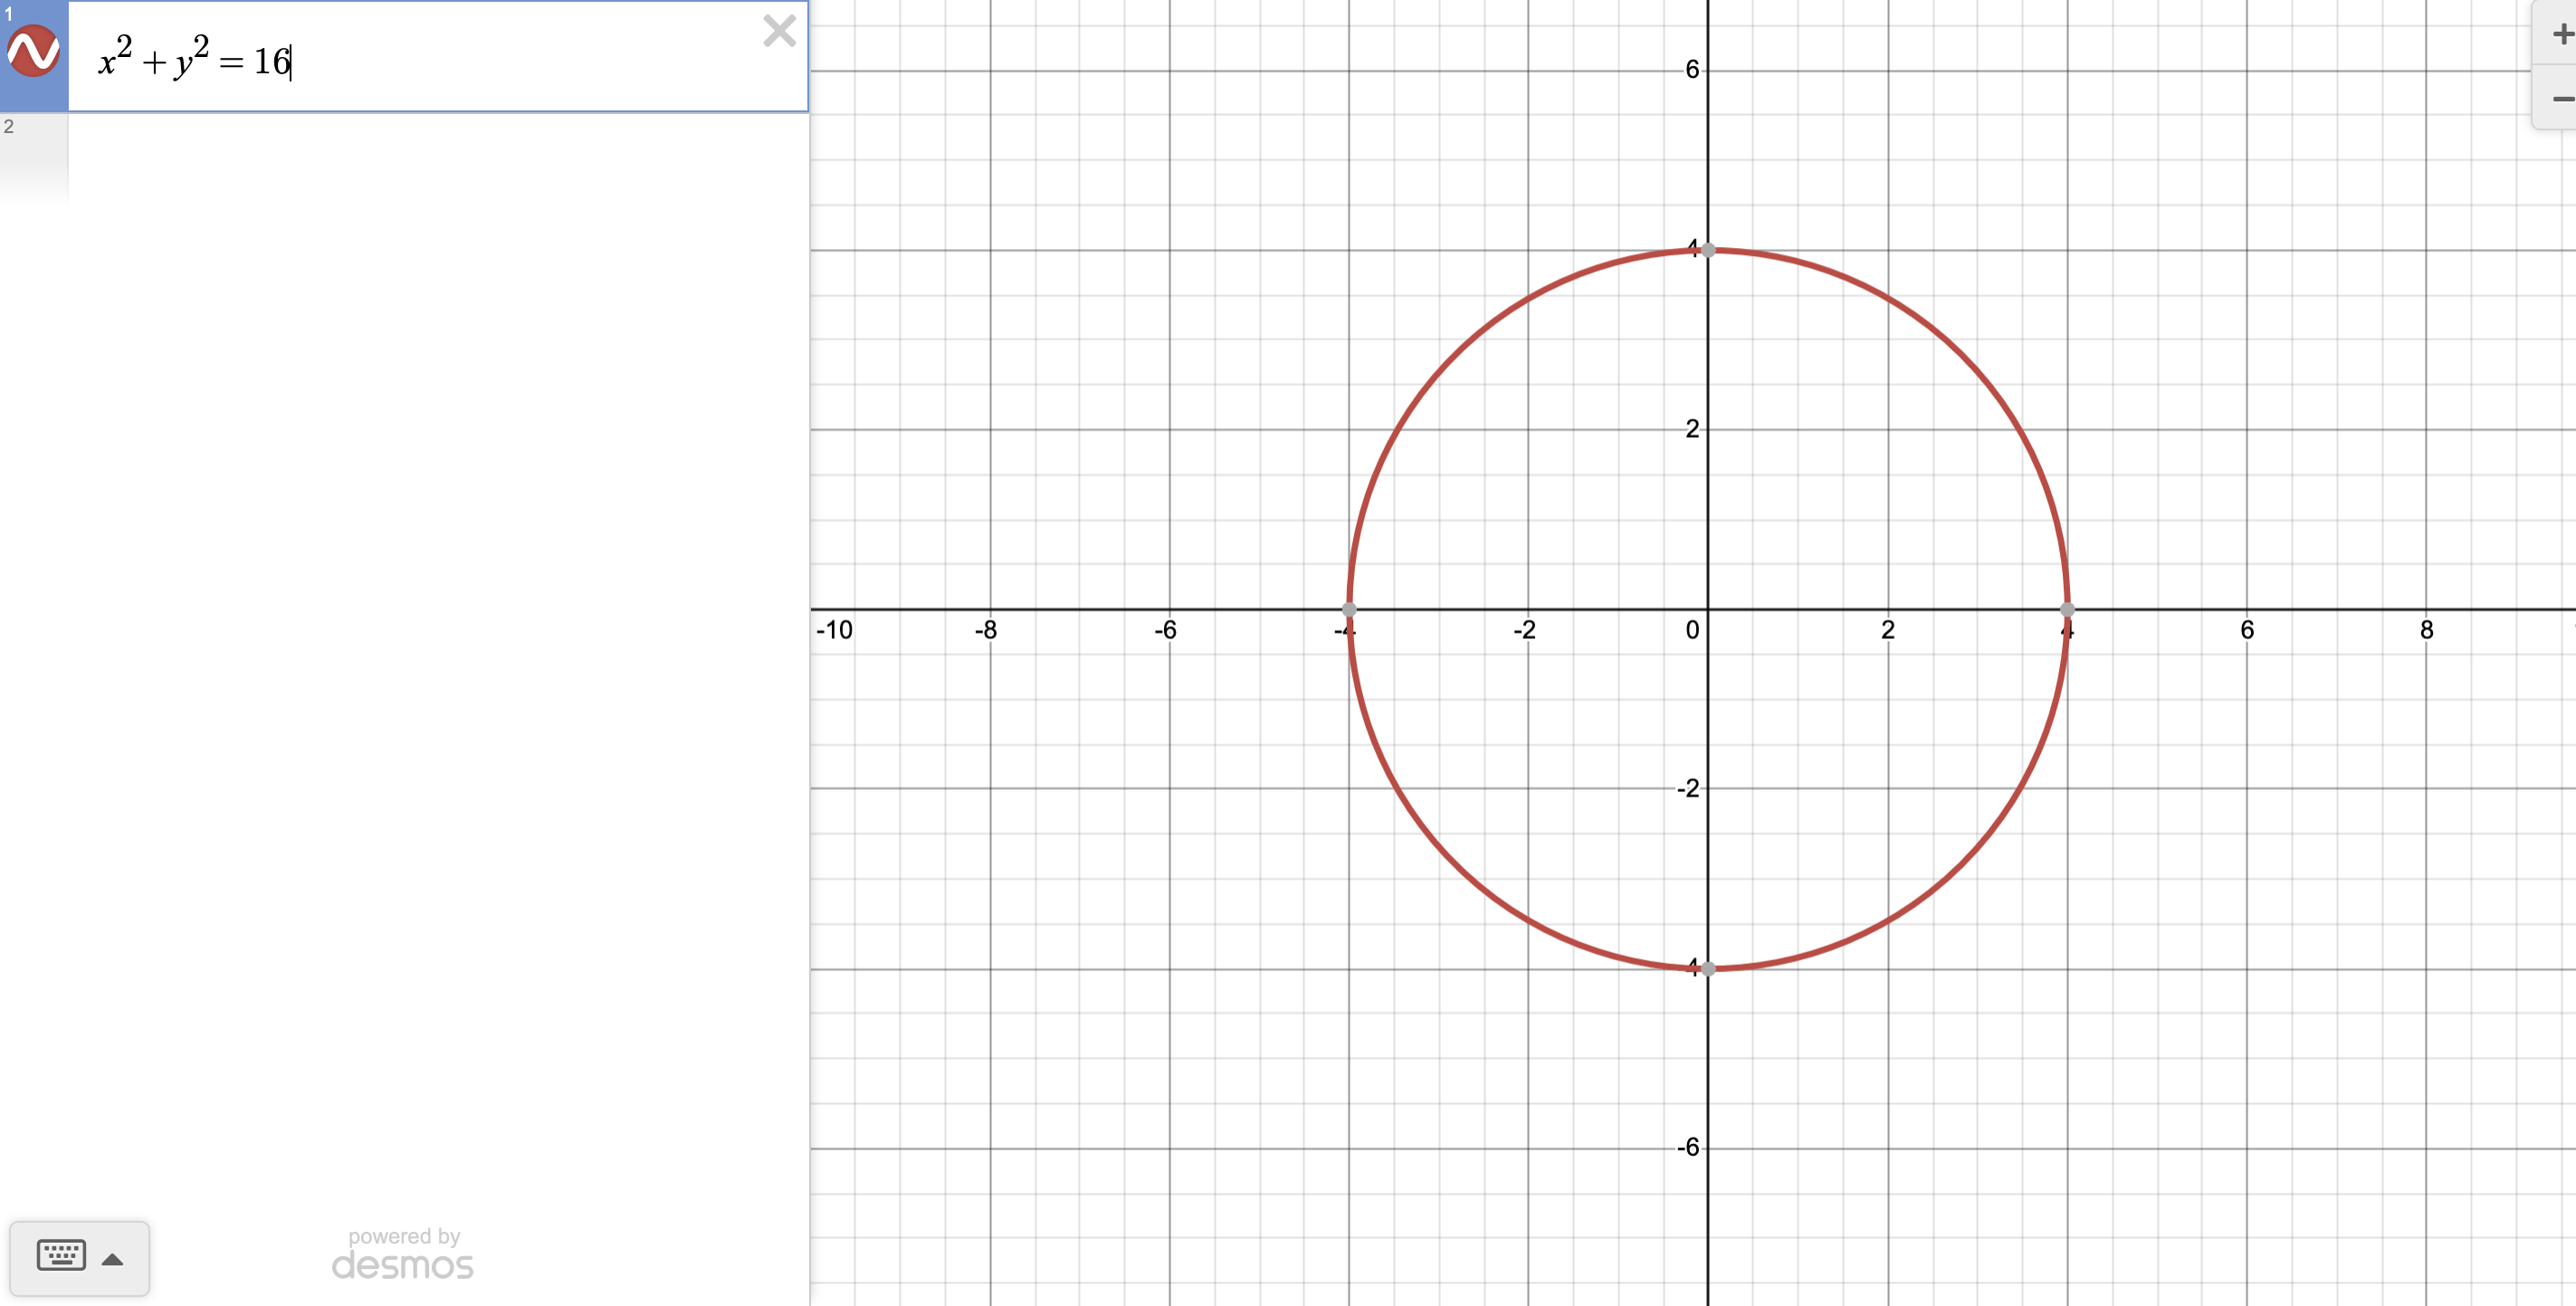
\includegraphics[width = 4in]{8}

\section*{9}
We are given the equation \[ 64y^2-x^2=64 \] \[ y^2-\frac{x^2}{8^2}=1 \] meaning this is a hyperbola with a vertical transverse axis. Also, $a=\sqrt{1}=1$ and 
$b=8$. Thus \[ c^2=1^2+8^2 \] \[ c=\sqrt{82} \] meaning the vertices are $(0,\pm 1)$ and the foci are $(0,\pm\sqrt{82})$. Also, the asymptotes are 
$y=\pm\frac{1}{8}x$:\newline
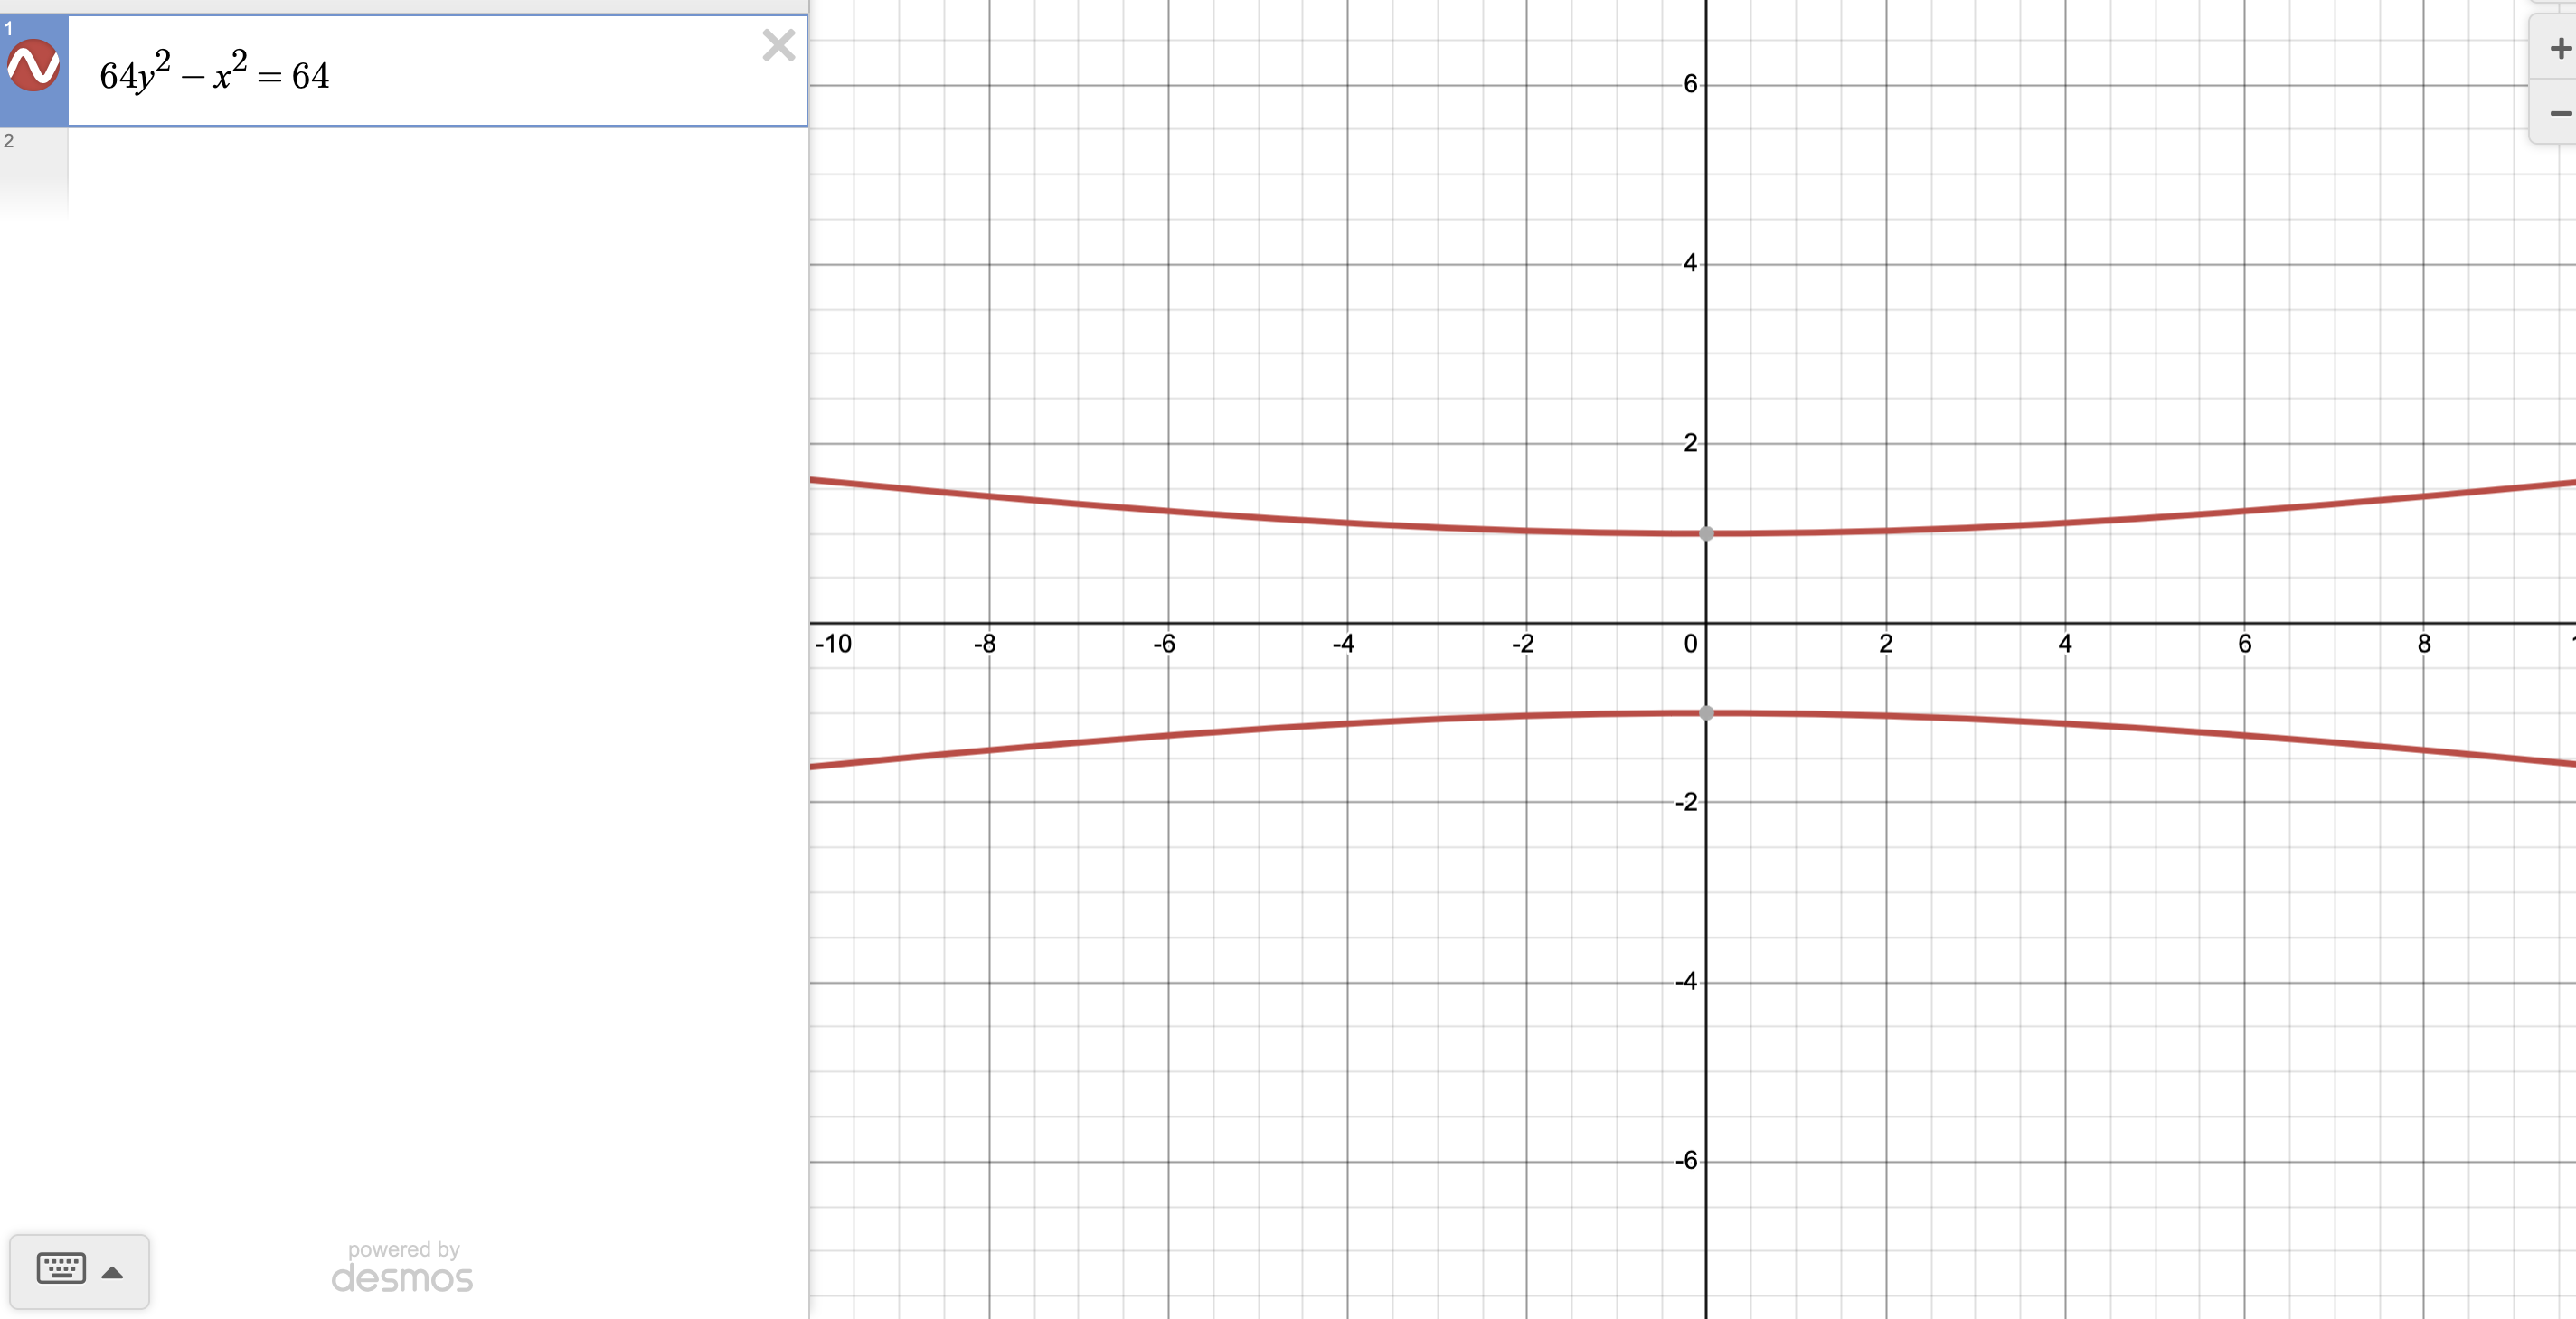
\includegraphics[width = 4in]{9}

\section*{10}
We are given the equation \[ 18x^2+2y^2=18 \] \[ x^2+\frac{y^2}{3^2}=1 \] meaning this is an ellipse with a vertical major axis. Also, $a=3$ and $b=\sqrt{1}=1$. 
Thus \[ c^2=3^2-1^2 \] \[ c=\sqrt{8}=2\sqrt{2} \] meaning the vertices are $(0,\pm 3)$, the co-vertices are $(\pm 1,0)$, and the foci are $(0,\pm 2\sqrt{2})$:\newline
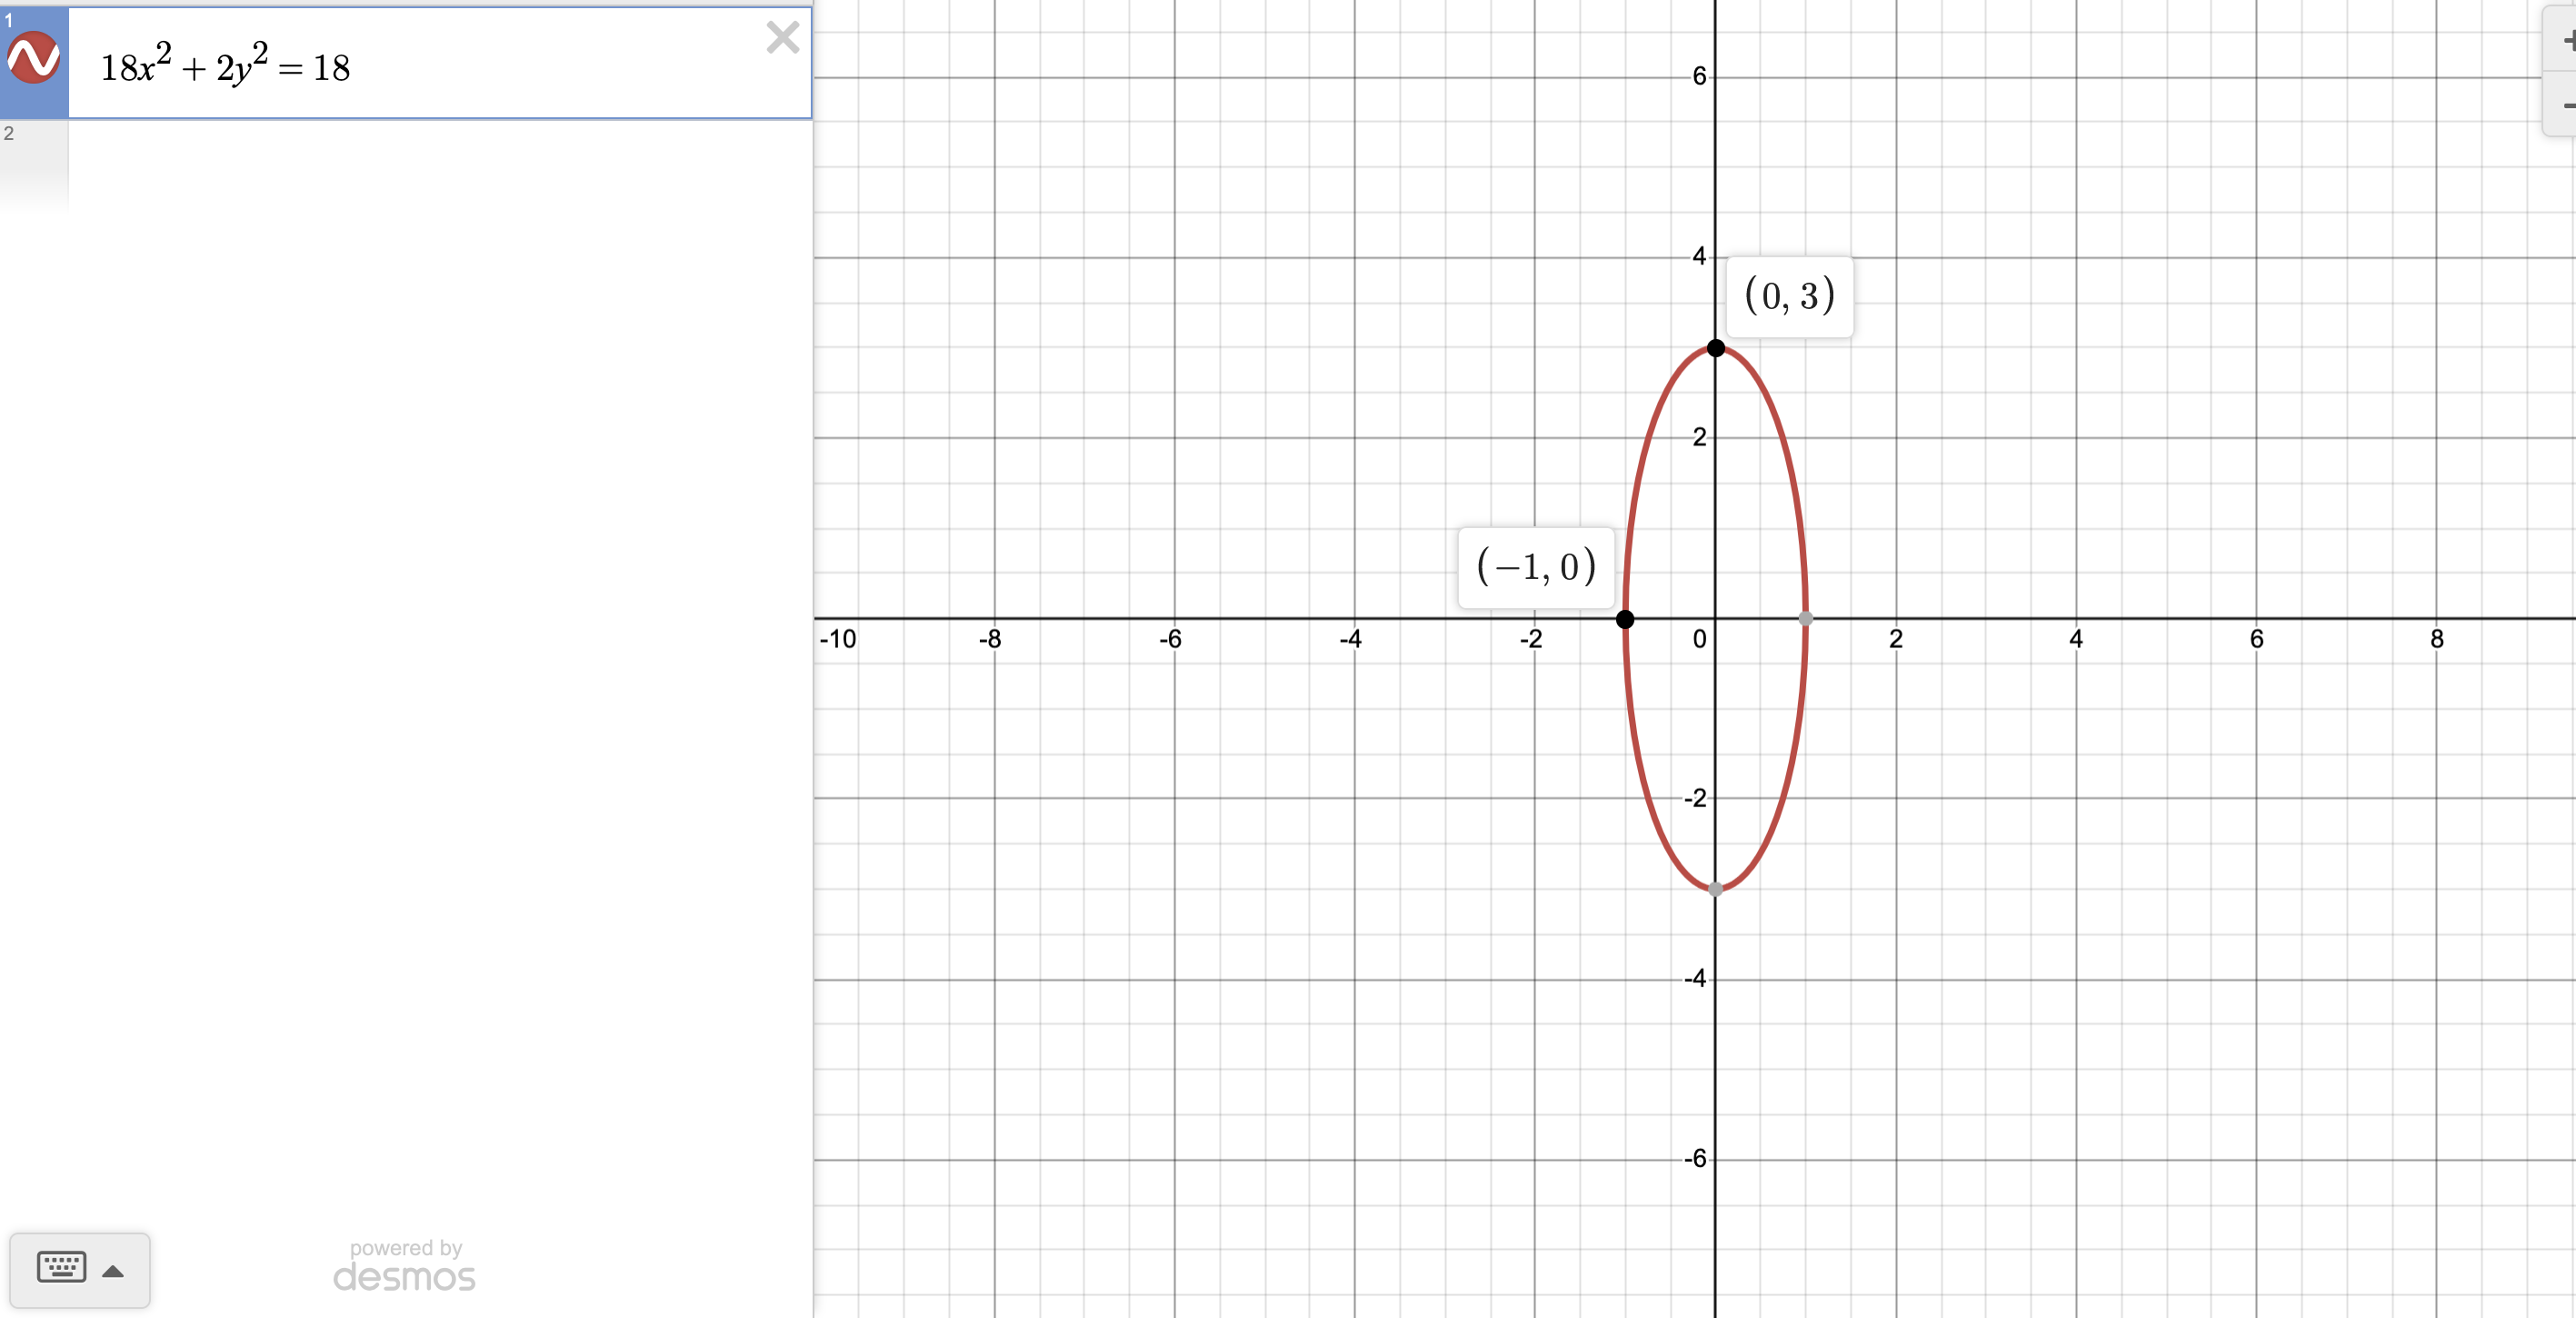
\includegraphics[width = 4in]{10}

\section*{11}
We are given the equation \[ (x-6)^2+(y+1)^2=36 \] This is a circle centered at $(6,-1)$ with a radius of 6:\newline
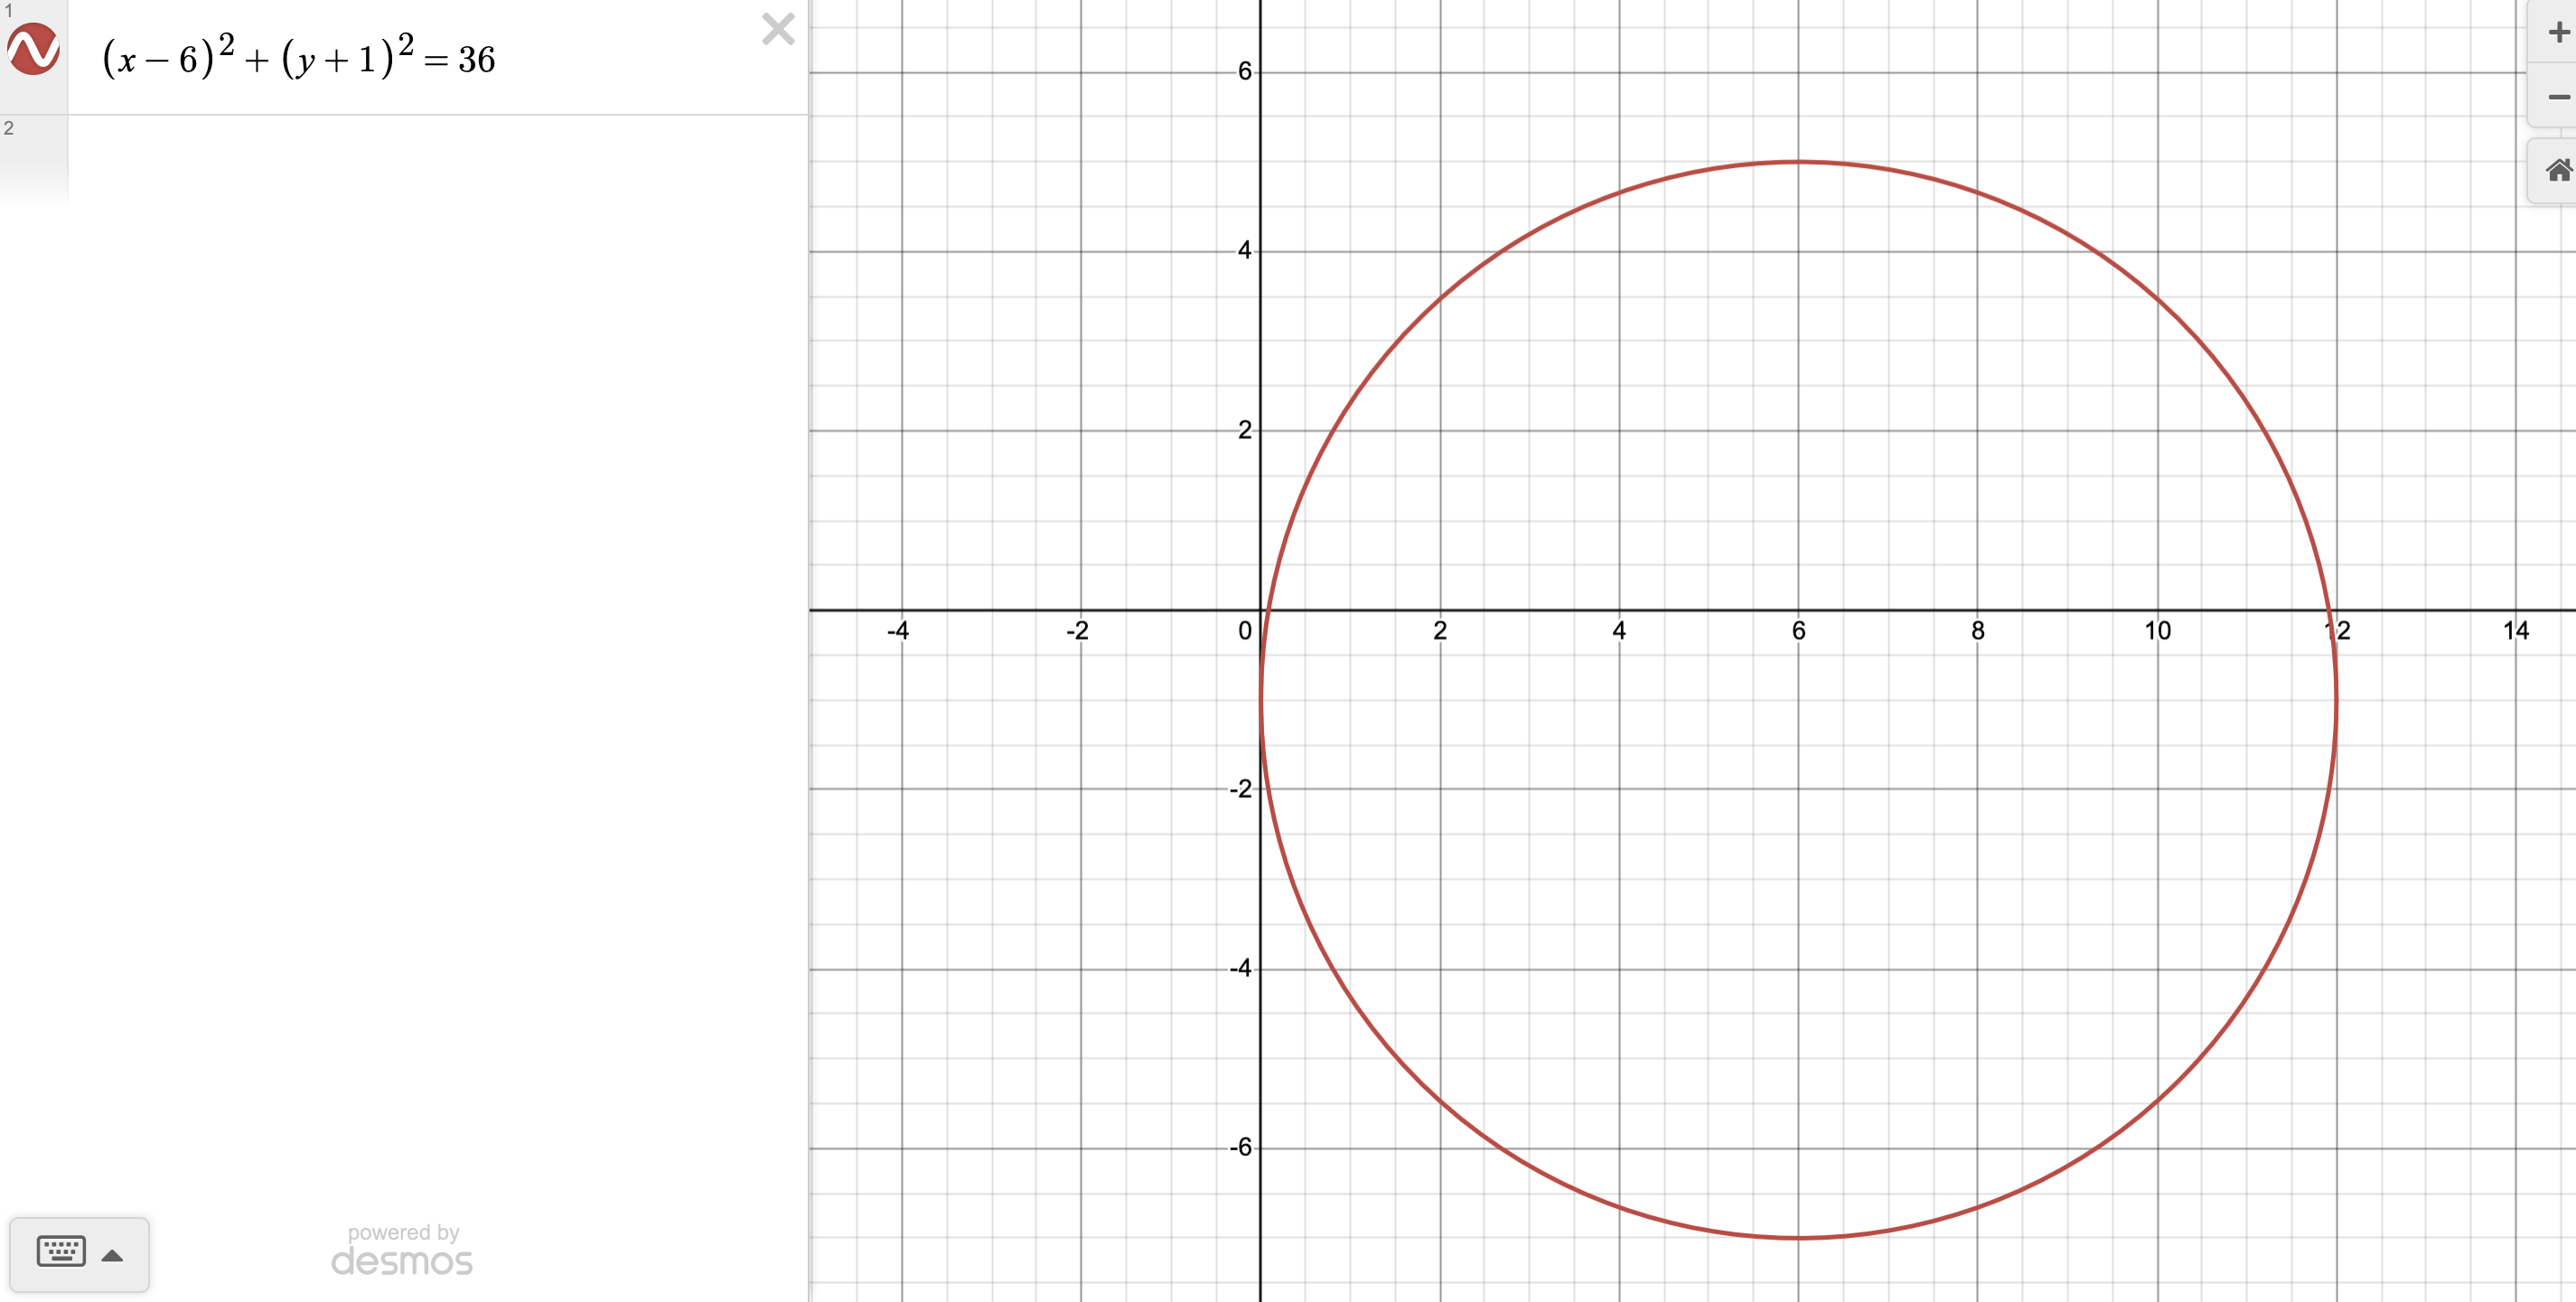
\includegraphics[width = 4in]{11}

\section*{12}
We are given the equation \[ (x+4)^2=6(y-2) \] This is a parabola with a vertex of $(-4,2)$ and a vertical axis of symmetry. 
We know that $p=\frac{6}{4}=\frac{3}{2}$ meaning the parabola has a focus of $(-4,2+\frac{3}{2})=(-4,\frac{7}{2})$ and a directrix of \[ y=2-\frac{3}{2} \]
\[ y=\frac{1}{2} \]
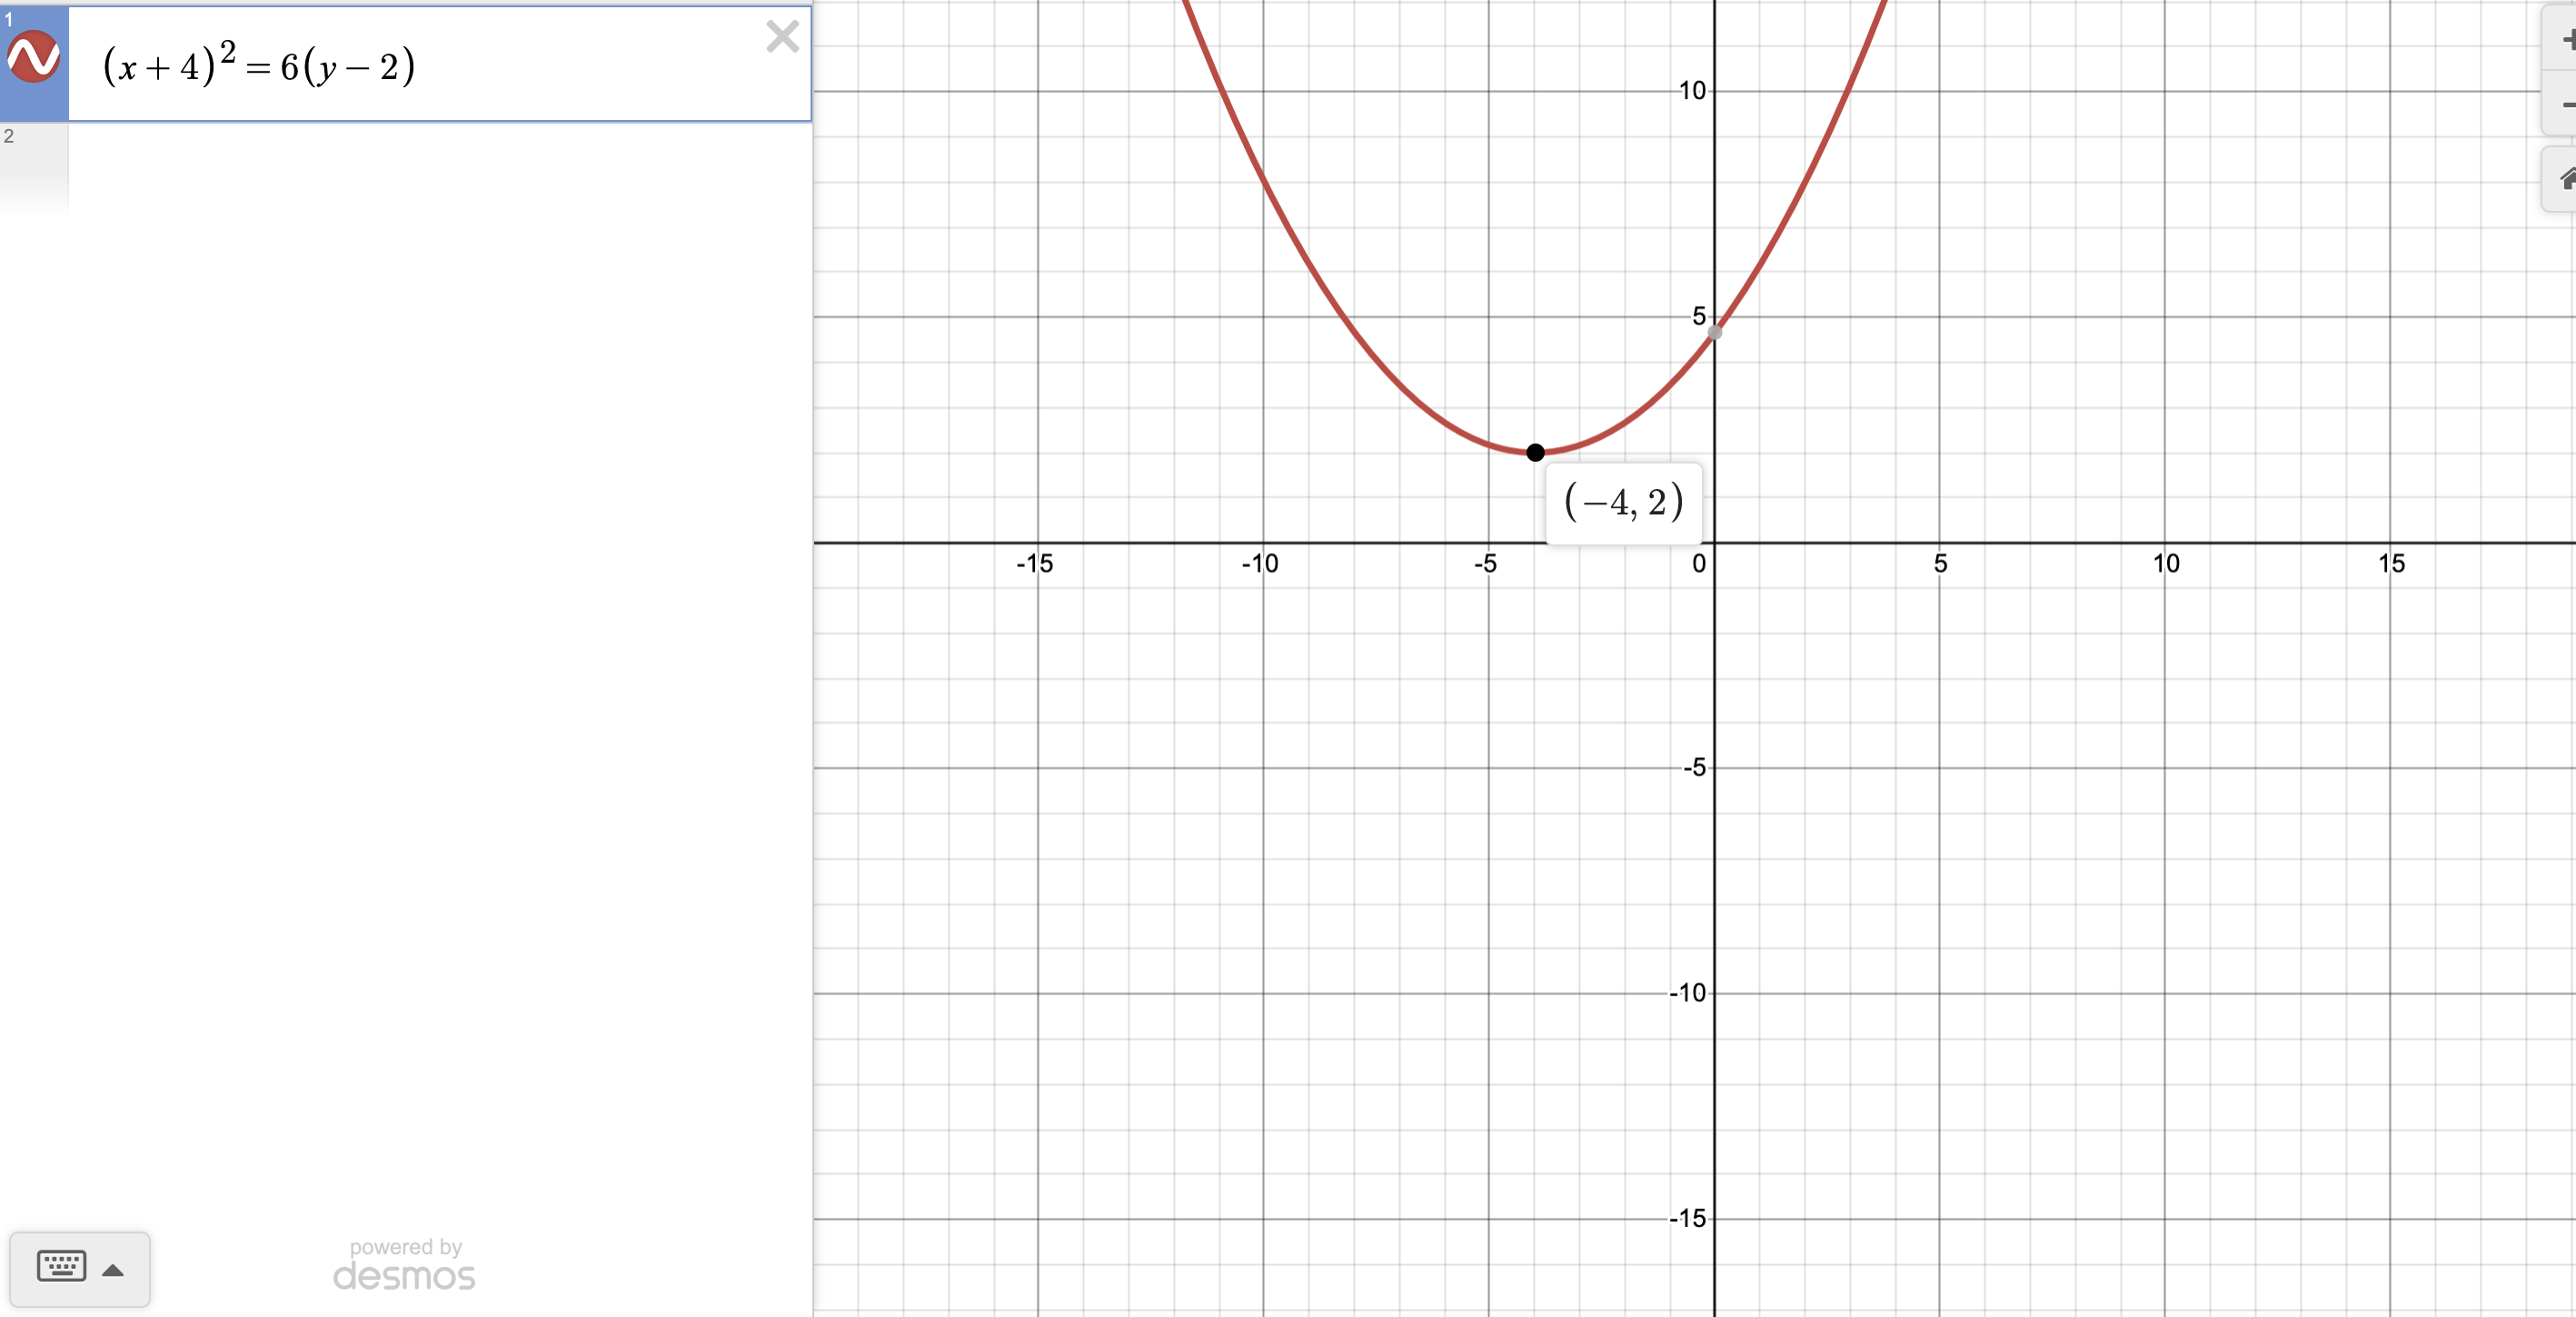
\includegraphics[width = 4in]{12}

\section*{13}
(I was unsure if the formulas for the asymptotes in the book given for hyperbola's centered at the origin also apply for hyperbolas centered on points other than the origin)\newline
We are given the equation \[ \frac{(x+4)^2}{9}-\frac{(y-7)^2}{49}=1 \] meaning this is a hyperbola centered at $(-4,7)$ with a horizontal transverse axis. Also, 
$a=3$ and $b=7$, meaning:
\[ c^2=3^2+7^2 \] \[ c=\sqrt{58} \] meaning the vertices are $(-4\pm 3,7)$ and the foci are $(-4\pm\sqrt{58},7)$:\newline
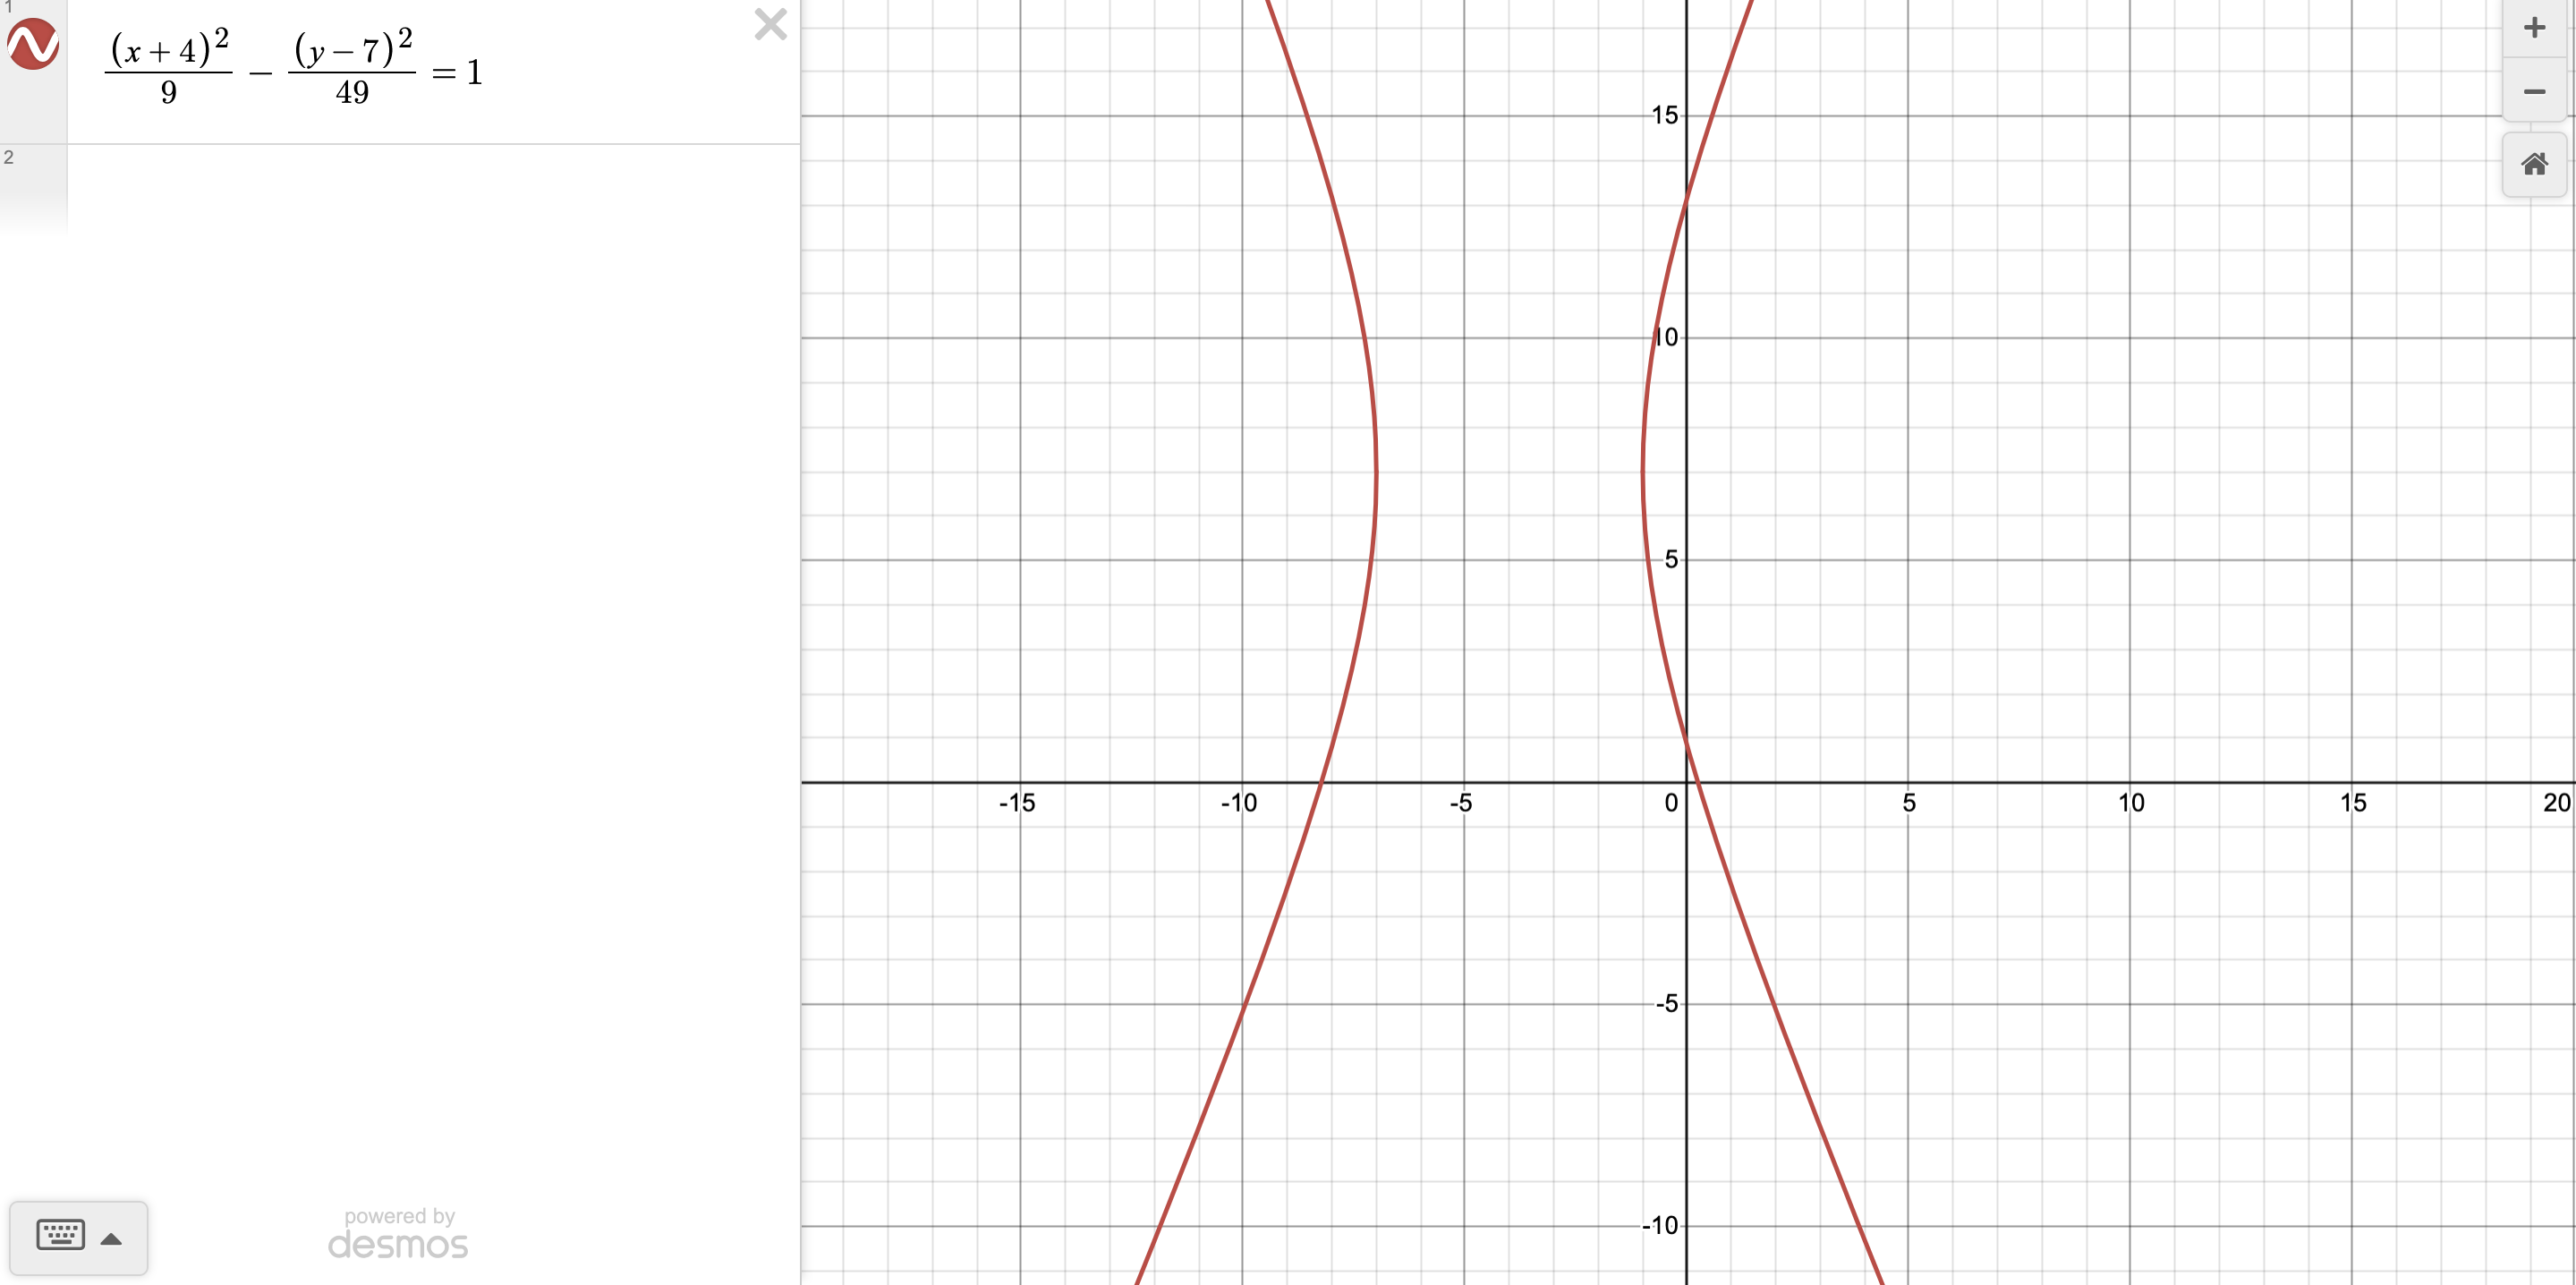
\includegraphics[width = 4in]{13}

\section*{14}
We are given the equation \[ \frac{(x-8)^2}{81}+\frac{(y-2)^2}{100}=1 \] which is an ellipse with a vertical major axis centered at $(8,2)$. We know that 
$a=10$ and $b=9$, meaning:
\[ c^2=10^2-9^2 \] \[ c=\sqrt{19} \] and thus the vertices are $(8,2\pm 10)$, the co-vertices are $(8\pm 9,2)$, and the foci are $(8,2\pm\sqrt{19})$:\newline
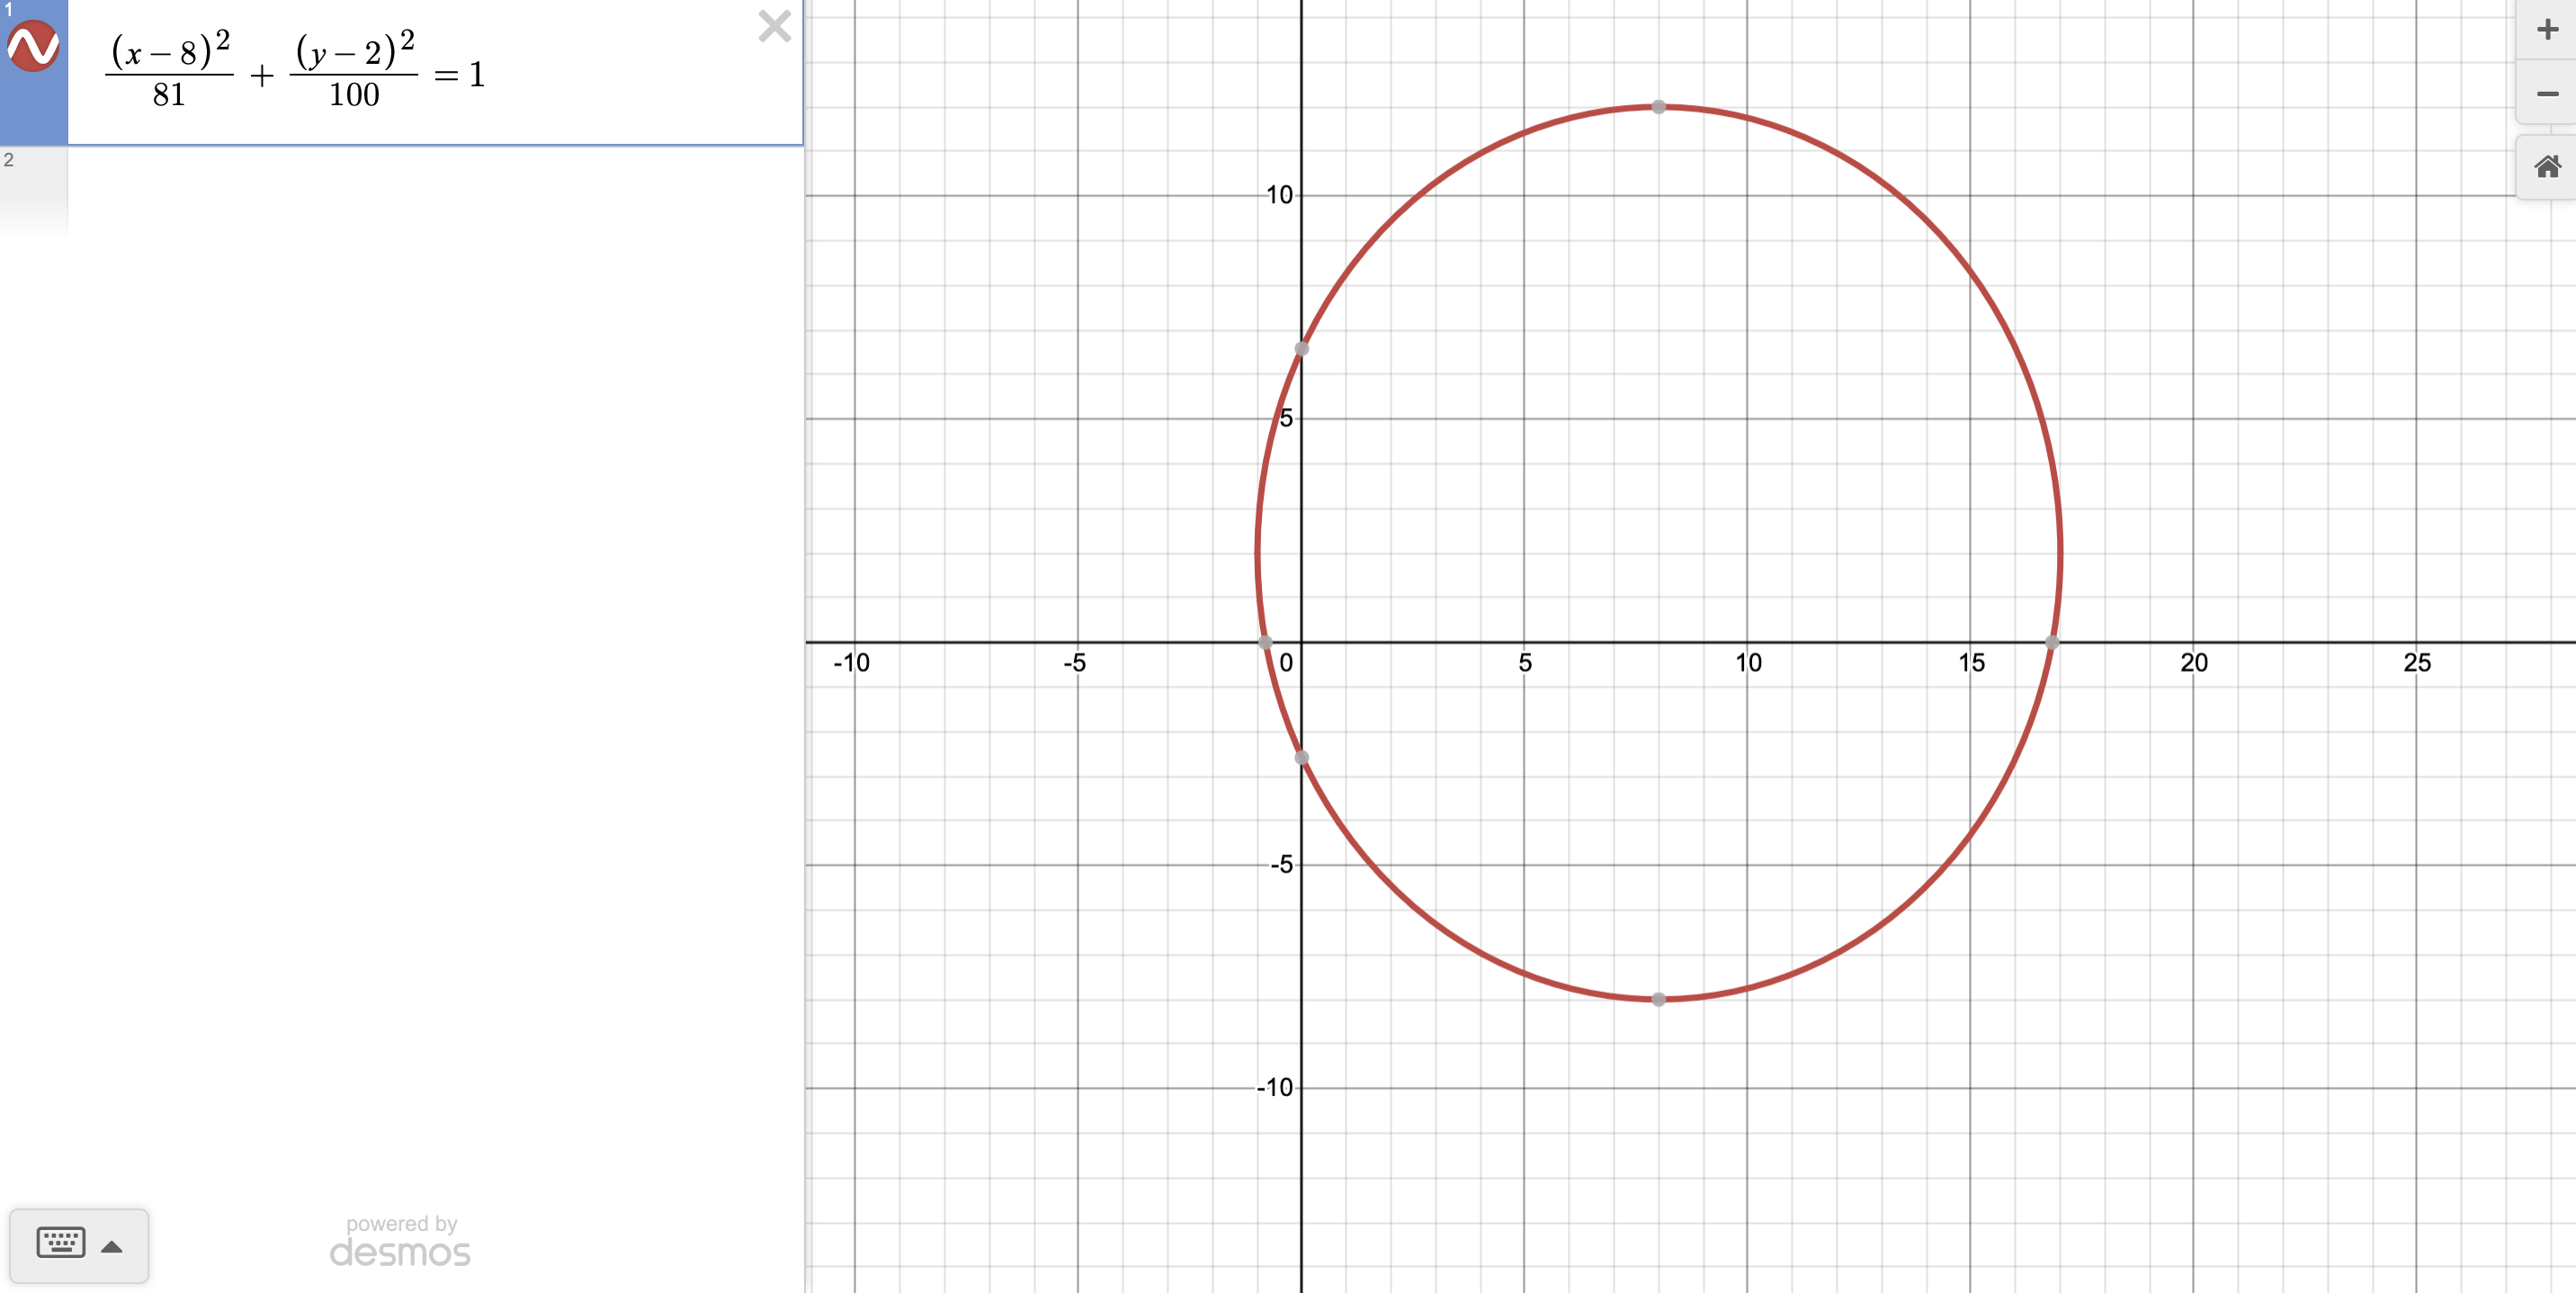
\includegraphics[width = 4in]{14}

\section*{15}
We are given the equation \[ \frac{(y-5)^2}{9}-(x+3)^2=1 \] meaning this is a hyperbola with a vertical transverse axis centered at $(-3,5)$. We know that 
$a=3$ and $b=1$, meaning:
\[ c^2=3^2+1^2 \] \[ c=\sqrt{10} \] and thus the vertices are $(-3,5\pm 3)$ and the foci are $(-3,5\pm\sqrt{10})$:\newline
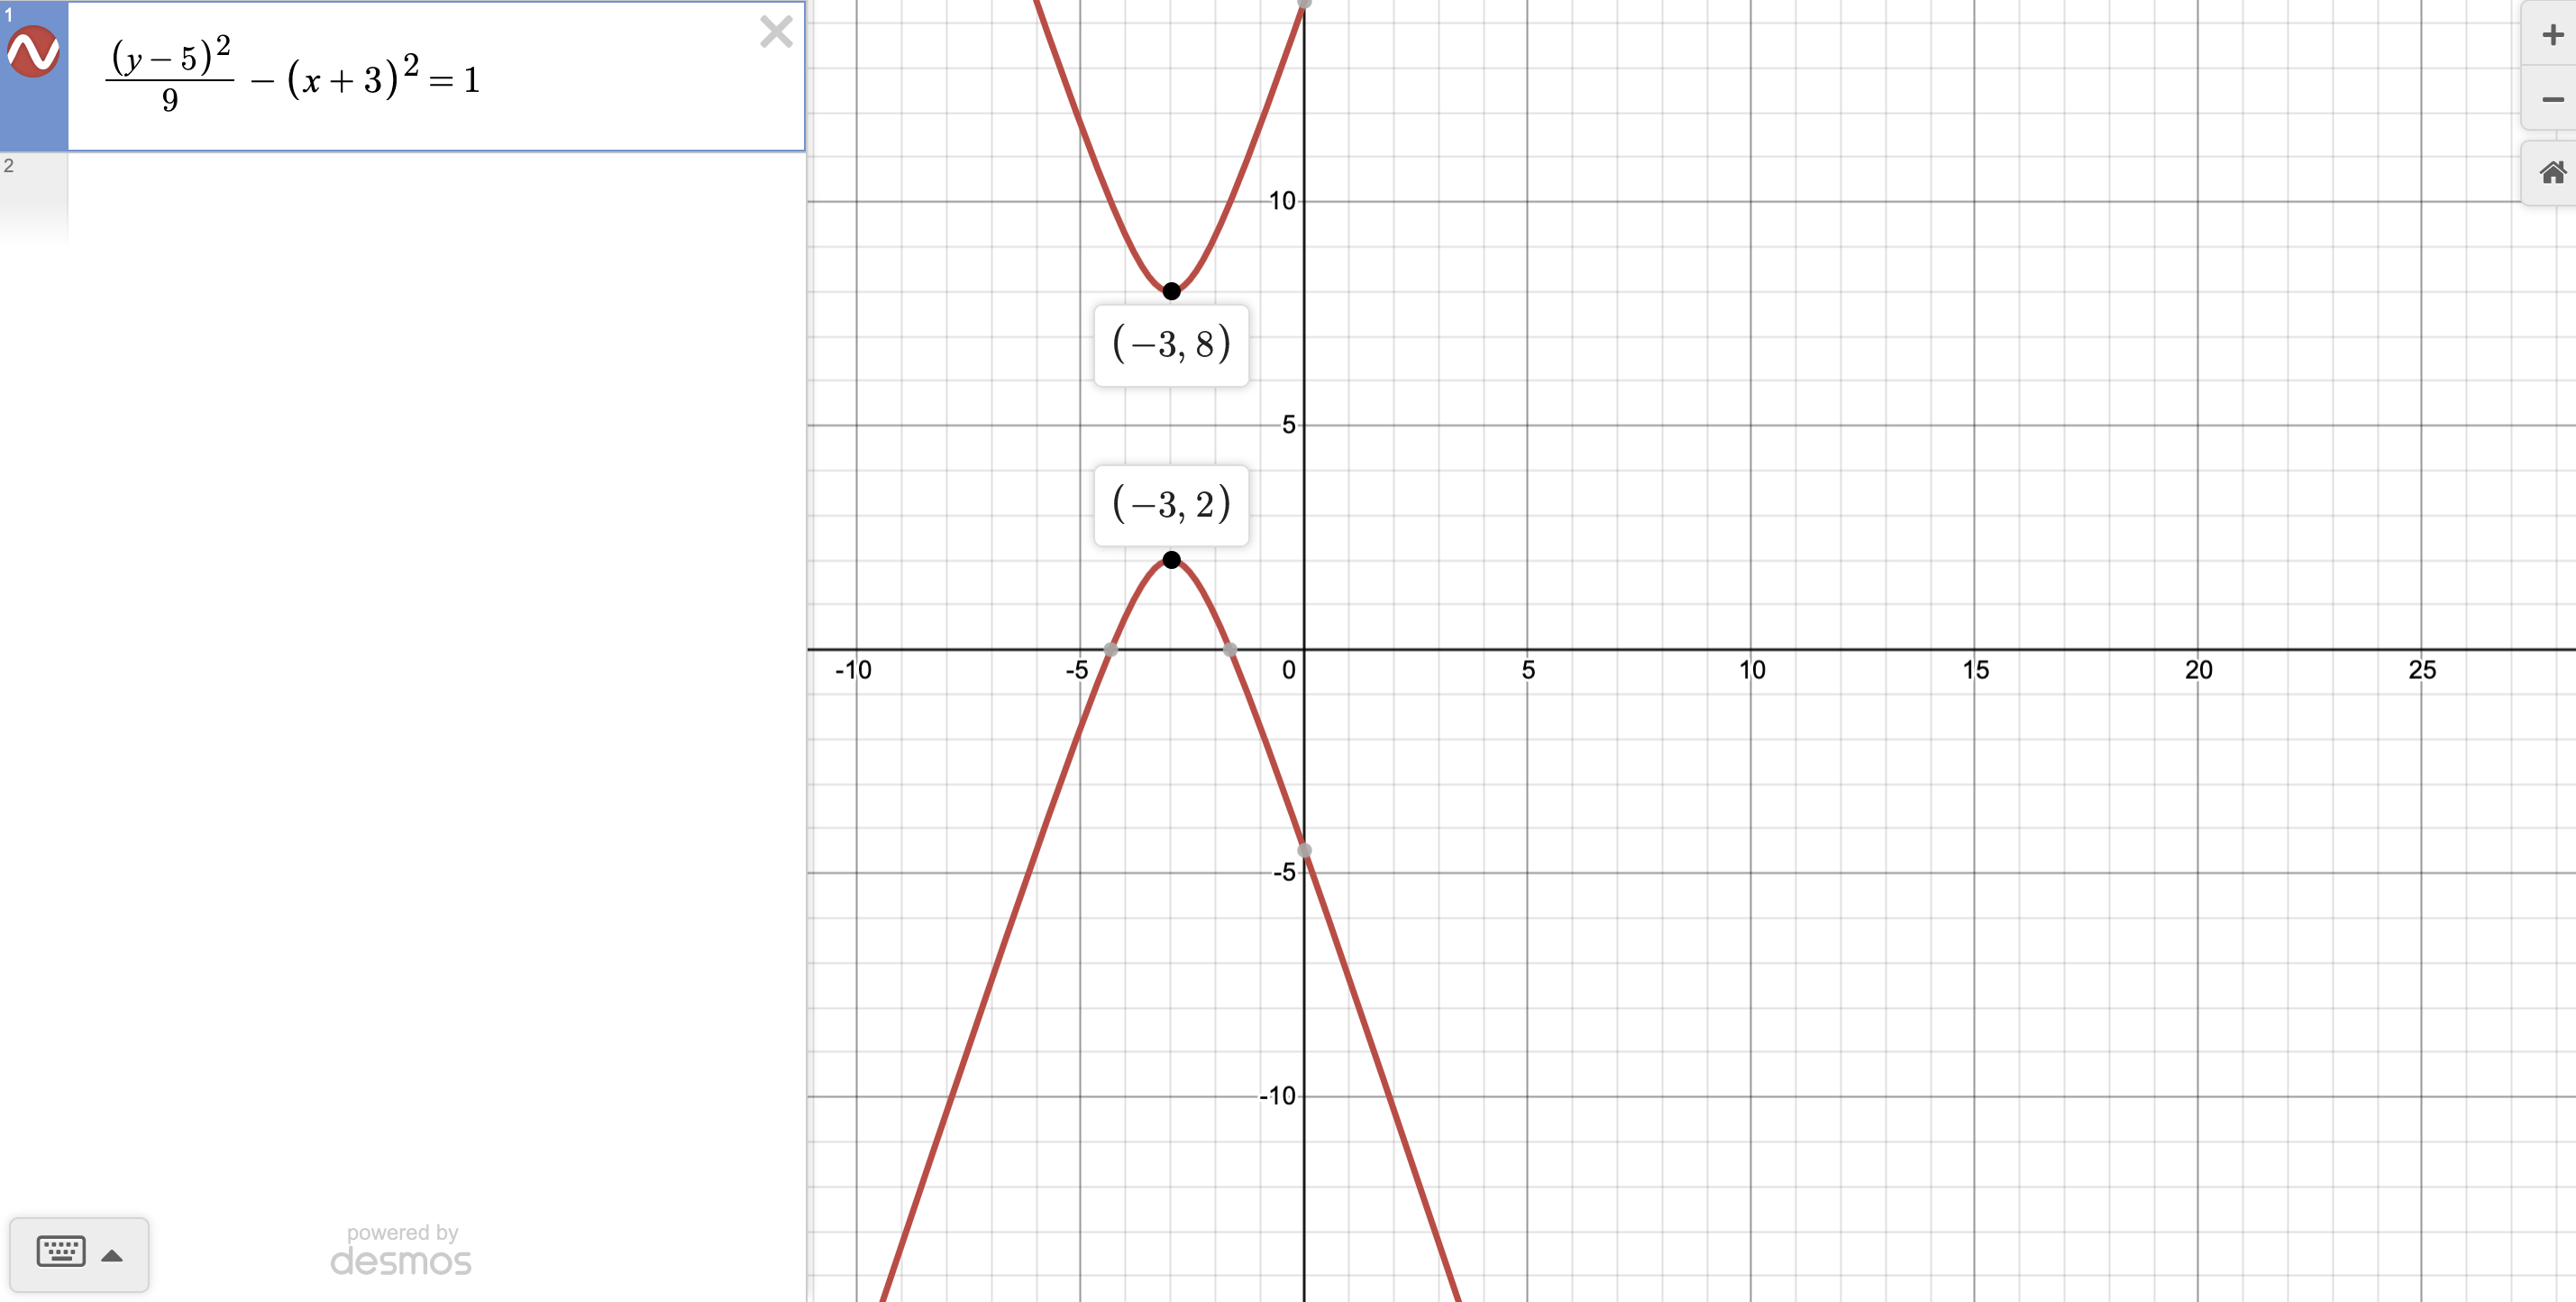
\includegraphics[width = 4in]{15}

\section*{16}
We are given a parabola with vertex at $(0,0)$ and directrix at $x=-6$. Hence $p=6$ and the axis of symmetry is horizontal, meaning the equation is:
\[ y^2=4(6)x \] \[ y^2=24x \]

\section*{17}
We are given a parabola with vertex at $(-2,-1)$ and focus at $(-2,5)$. Thus we know that $p=|5+1|=6$ and the axis of symmetry is vertical meaning the equation is:
\[ (x+2)^2=24(y+1) \]

\section*{18}
We are given a circle with center $(0,0)$ and passing through $(-5,2)$. We can find the radius by finding the distance from $(-5,2)$ to $(0,0)$:
\[ \sqrt{(0+5)^2+(0-2)^2}=\sqrt{25+4}=\sqrt{29} \] meaning the radius is $\sqrt{29}$ and thus the equation for the circle is:
\[ x^2+y^2=29 \]

\section*{19}
We are given a circle with center $(1,-4)$ and radius 6, meaning the equation for the circle is:
\[ (x-1)^2+(y+4)^2=6^2 \]

\section*{20}
We are given an ellipse with center at $(0,0)$, vertex at $(0,6)$, and co-vertex at $(-3,0)$. Thus the major axis is vertical, 
$a=6$, and $b=3$, meaning the equation is:
\[ \frac{x^2}{9}+\frac{y^2}{36}=1 \]

\section*{21}
We are given an ellipse with vertices at $(-1,4)$ and $(7,4)$ and foci at $(1,4)$ and $(5,4)$. We know that the center is halfway between the two vertices, meaning it is located at
\[ (\frac{-1+7}{2},\frac{4+4}{2})=(3,4) \] and the major axis is horizontal. Thus $a=4$ and $c=2$, meaning:
\[ b^2=4^2-2^2 \] \[ b=\sqrt{12}=2\sqrt{3} \] meaning the equation for the ellipse is:
\[ \frac{(x-3)^2}{16}+\frac{(y-4)^2}{12}=1 \]

\section*{22}
We are given a hyperbola with vertices at $(0,-6)$ and $(0,6)$ and foci at $(0,-9)$ and $(0,9)$. We know that the center is halfway between the vertices; hence it is 
$(0,0)$, and the transverse axis is vertical. Thus $a=6$ and $c=9$, meaning:
\[ b^2=9^2-6^2 \] \[ b=\sqrt{55} \] meaning the equation for the hyperbola is
\[ \frac{y^2}{36}-\frac{x^2}{55}=1 \]

\section*{23}
We are given a hyperbola with a vertex at $(2,-5)$, focus at $(-1,-5)$, and center at $(5,-5)$. Thus $a=3$ and $c=6$ and the transverse axis is horizontal. Thus
\[ b^2=6^2-3^2 \] \[ b=\sqrt{27}=3\sqrt{3} \] meaning the equation for the hyperbola is
\[ \frac{x^2}{9}-\frac{y^2}{27}=1 \]

\section*{24}
We know that $B^2-4AC=0^2-4(1)(4)<0$, and because $A\ne C$, the equation is an ellipse. To write the equation in standard form, we need to complete the square:
\[ x^2+4y^2-6x-16y+21=0 \]
\[ (x^2-6x+9)+4(y^2-4y+4)+21=9+16 \]
\[ (x-3)^2+4(y-2)^2+21=25 \]
\[ \frac{(x-3)^2}{4}+(y-2)^2=1 \]

\section*{25}
We know that $B^2-4AC=0^2-4(1)(1)<0$, and because $B=0$ and $A=C$, the equation is a circle. To write the equation in standard form, we need to complete the square:
\[ x^2+y^2+8x+12y+3=0 \]
\[ (x^2+8x+16)+(y^2+12y+36)+3=16+36 \]
\[ (x+4)^2+(y+6)^2+3=52 \]
\[ (x+4)^2+(y+6)^2=49=7^2 \]

\section*{26}
We know that $B^2-4AC=0^2-4(4)(-9)>0$ meaning the equation is a hyperbola. To write the equation in standard form, we need to complete the square:
\[ 4x^2-9y^2-40x+64=0 \]
\[ 4(x^2-10x+25)-9y^2+64=100 \]
\[ 4(x-5)^2-9y^2=36 \]
\[ \frac{(x-5)^2}{9}-\frac{y^2}{4}=1 \]

\section*{27}
We know that $B^2-4AC=0^2-4(0)(1)=0$ meaning the equation is parabola. To write the equation in standard form, we need to complete the square:
\[ y^2-16y-12x+40=0 \]
\[ (y^2-16y+64)=12x-40+64 \]
\[ (y-8)^2=12(x+2) \]

\section*{28}
We know that $B^2-4AC=0^2-4(25)(4)<0$ and because $A\ne C$, the equation is an ellipse. To write the equation in standard form, we need to complete the square:
\[ 25x^2+4y^2+50x-24y-39=0 \]
\[ 25(x^2+2x+1)+4(y^2-6y+9)-39=25+36 \]
\[ 25(x+1)^2+4(y-3)^2=100 \]
\[ \frac{(x+1)^2}{4}+\frac{(y-3)^2}{25}=1 \]

\section*{29}
We know that $B^2-4AC=0^2-4(-16)(1)>0$ meaning the equation is a hyperbola. To write the equation in standard form, we need to complete the square:
\[ y^2-16x^2+14y+64x-31=0 \]
\[ -16(x^2-4x+4)+(y^2+14y+49)-31=-64+49 \]
\[ -16(x-2)^2+(y+7)^2=16 \]
\[ -(x-2)^2+\frac{(y+7)^2}{16}=1 \]
\[ \frac{(y+7)^2}{16}-(x-2)^2=1 \]

\section*{30}
\[ x+y=2 \] \[ x=2-y \] meaning
\[ 4x^2+y^2=16 \] \[ 4(2-y)^2+y^2=16 \]
\[ 4(4-4y+y^2)+y^2=16 \]
\[ 16-16y+4y^2+y^2=16 \]
\[ 5y^2-16y=0 \]
\[ y(5y-16)=0 \]
\[ y=0\vee y=\frac{16}{5} \]
and \[ x=2-0=2\vee x=2-\frac{16}{5}=-\frac{6}{5} \]

\section*{31}
Because $y^2-2y-8x-16=0$, $-4y^2+8y+32x+64=0$ and thus
\[ (x^2+4y^2-8y-4)+(-4y^2+8y+32x+64)=0 \]
\[ x^2+32x+60=0 \]
\[ (x+30)(x+2)=0 \]
\[ x=-30\vee x=-2 \]
and \[ y^2-2y-8(-30)-16=0 \]
\[ y^2-2y+224=0 \]
\[ y=\frac{2\pm\sqrt{(-2)^2-4(1)(224)}}{2(1)} \]
\[ =\frac{2\pm\sqrt{-892}}{2} \]
\[ =\frac{2\pm 2i\sqrt{223}}{2} \]
for $x=-30$ and
\[ y^2-2y-8(-2)-16=0 \]
\[ y^2-2y=0 \]
\[ y(y-2)=0 \]
\[ y=0\vee y=2 \]
for $x=-2$.

\section*{32}
\[ (y^2-x^2+2x-5)+(x^2+y^2-2x-3)=0 \]
\[ 2y^2-8=0 \]
\[ y^2-4=0 \]
\[ y=\pm 2 \]
and \[ x^2+(\pm 2)^2-2x-3=0 \]
\[ x^2-2x+1=0 \]
\[ (x-1)^2=0 \]
\[ x=1 \] for $y=\pm 2$.

\section*{33}
(I was not entirely sure whether the major axis was vertical or horizontal for the ellipse)\newline
We let the center of the water's surface be the origin. When the glass is upright, the water's surface is a cirlce with radius 1.5 inches, meaning it has the equation
$x^2+y^2=1.5^2$. When it is tilted, it becomes an ellipse with minor axis 3 inches long and major axis 6 inches long, and a horizontal major axis. Thus it can be modeled by the equation 
$\frac{x^2}{36}+\frac{y^2}{9}=1$.

\section*{34}
We are given one point on the parabola: $(-104,45)$. Thus we can solve for $p$:
\[ (-104)^2=4p(45) \]
\[ p=\frac{2704}{45} \]
meaning an equation for the parabola is \[ x^2=4\frac{2704}{45}y=\frac{10816}{45}y \]
Because $p=\frac{10816}{45}$ and the axis of symmetry is vertical, the focus is $(0,\frac{10816}{45})$. Thus the distance from the vertex to the focus is 
$\frac{10816}{45}$.

\end{document}
